%% -*- coding: utf-8 -*-
\documentclass[12pt,a4paper]{scrartcl} 
\usepackage[utf8]{inputenc}
\usepackage[english,russian]{babel}
\usepackage{indentfirst}
\usepackage{misccorr}
\usepackage{graphicx}
\usepackage{amsmath}
\begin{document}
	\begin{titlepage}
		\begin{center}
			\large
			МИНИСТЕРСТВО НАУКИ И ВЫСШЕГО ОБРАЗОВАНИЯ РОССИЙСКОЙ ФЕДЕРАЦИИ
			
			Федеральное государственное бюджетное образовательное учреждение высшего образования
			
			\textbf{АДЫГЕЙСКИЙ ГОСУДАРСТВЕННЫЙ УНИВЕРСИТЕТ}
			\vspace{0.25cm}
			
			Инженерно-физический факультет
			
			Кафедра автоматизированных систем обработки информации и управления
			\vfill

			\vfill
			
			\textsc{Отчет по практике}\\[5mm]
			
			{\LARGE \textit{Сортировки Быстрая и Слиянием}}
			\bigskip
			
			2 курс, группа 2УТС
		\end{center}
		\vfill
		
		\newlength{\ML}
		\settowidth{\ML}{«\underline{\hspace{0.7cm}}» \underline{\hspace{2cm}}}
		\hfill\begin{minipage}{0.5\textwidth}
			Выполнил:\\
			\underline{\hspace{\ML}} О.\,Д.~Козырев\\
			«\underline{\hspace{0.7cm}}» \underline{\hspace{2cm}} 2022 г.
		\end{minipage}%
		\bigskip
		
		\hfill\begin{minipage}{0.5\textwidth}
			Руководитель:\\
			\underline{\hspace{\ML}} С.\,В.~Теплоухов\\
			«\underline{\hspace{0.7cm}}» \underline{\hspace{2cm}} 2022 г.
		\end{minipage}%
		\vfill
		
		\begin{center}
			Майкоп, 2022 г.
		\end{center}
	\end{titlepage}
		
	\section{Введение}
	\label{sec:intro}
	\begin{enumerate}
	\item Текстовая формулировка задачи:
	
	Сортировки Быстрая и Слиянием.
	\item Код на языке C++ приведен в пункте~\ref{sec:exp:code} на стр.~\pageref{sec:exp:code}.
	\item Результат работы представлен в пункте~\ref{sec:result:screen} на стр.~\pageref{figure1:screen} и~\pageref{figure2:screen}.
	\end{enumerate}
	
	\section{Ход работы}
	\label{sec:exp}
	
	\subsection{Код программы}
	\label{sec:exp:code}
	\begin{verbatim}
	
#include <iostream>
#include <locale>
using namespace std;
int section(int mas[], int nachalo, int end) {
    int point = mas[nachalo];
    int count = 0;
    for (int i = nachalo + 1; i <= end; i++) {
        if (mas[i] <= point)
            count++;}
    int in = nachalo + count;
    swap(mas[in], mas[nachalo]);
    int i = nachalo, j = end;
    while (i < in && j > in) {
        while (mas[i] <= point)
            i++;
        while (mas[j] > point)
            j--;
        if (i < in && j > in)
            swap(mas[i++], mas[j--]);}
    return in;}
void sortirovka(int mas[], int start, int end) {
    if (start >= end)
        return;
    int p = section(mas, start, end);
    sortirovka(mas, start, p - 1);
    sortirovka(mas, p + 1, end);}
void sort(int*, int, int, int);
void _sortirovka_(int* arr, int low, int high) {
    int mid;
    if (low < high) {
        mid = (low + high) / 2;
        _sortirovka_(arr, low, mid);
        _sortirovka_(arr, mid + 1, high);
        sort(arr, low, high, mid);}}
void sort(int* arr, int low, int high, int mid) {
    int i, j, k, c[50];
    i = low;
    k = low;
    j = mid + 1;
    while (i <= mid && j <= high) {
        if (arr[i] < arr[j]) {
            c[k] = arr[i];
            k++;
            i++;}
        else {
            c[k] = arr[j];
            k++;
            j++;}}
    while (i <= mid) {
        c[k] = arr[i];
        k++;
        i++;}
    while (j <= high) {
        c[k] = arr[j];
        k++;
        j++;}
    for (i = low; i < k; i++)
        arr[i] = c[i];}
int main() {
    setlocale(LC_ALL, "rus");
    int n;
    do {  cout << "количество элементов: ";
        cin >> n;
        if (n <= 0)
            cout << "ошибка" << endl;
    } while (n <= 0);
    int mas[100];
    cout << "введите элементы: ";
    for (int i = 0; i < n; i++)
        cin >> mas[i];
    int vibor;
    do { cout << "1 быстрая" << endl << "2 слиянием" << endl;
        cin >> vibor;
        if (vibor != 1 && vibor != 2)
            cout << "ошибка" << endl;
    } while (vibor != 1 && vibor != 2);
    switch (vibor) {
    case 1:
        sortirovka(mas, 0, n - 1);
        cout << "отсортированные элементы: ";
        for (int i = 0; i < n; i++)
            cout << mas[i] << " ";
        break;
    case 2:
        _sortirovka_(mas, 0, n - 1);
        cout << "отсортированные элементы: ";
        for (int i = 0; i < n; i++)
            cout << mas[i] << " ";
        break;}}
	
	\end{verbatim}
	
	\section{Результат работы программы}
	\label{sec:result}
	
	\subsection{Скриншоты выполнения кода}
	\label{sec:result:screen}
	\begin{figure}[h]
	\centering
	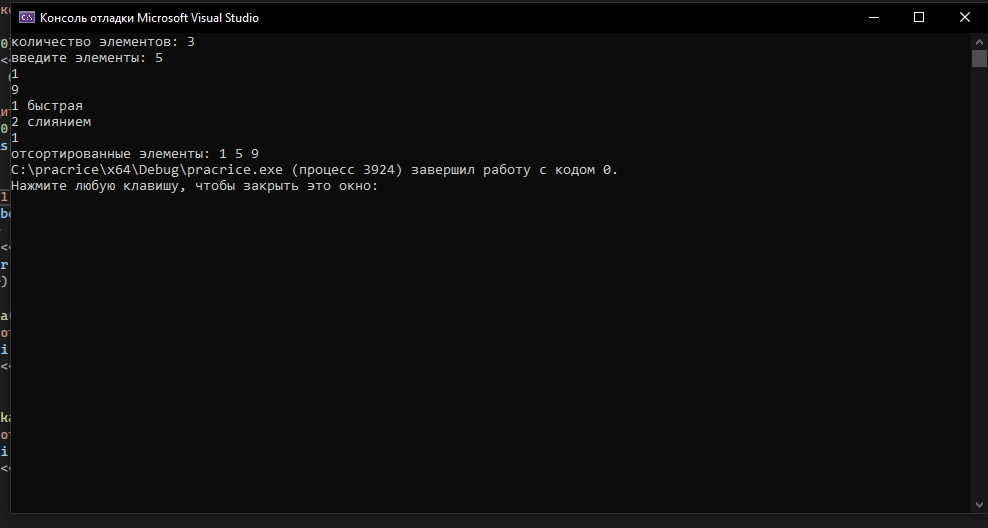
\includegraphics[width=1\textwidth]{skrin bis.jpg}
	\caption{Быстрая сортировка}\label{figure1:screen}
	\end{figure}

	\begin{figure}[h]
	\centering
	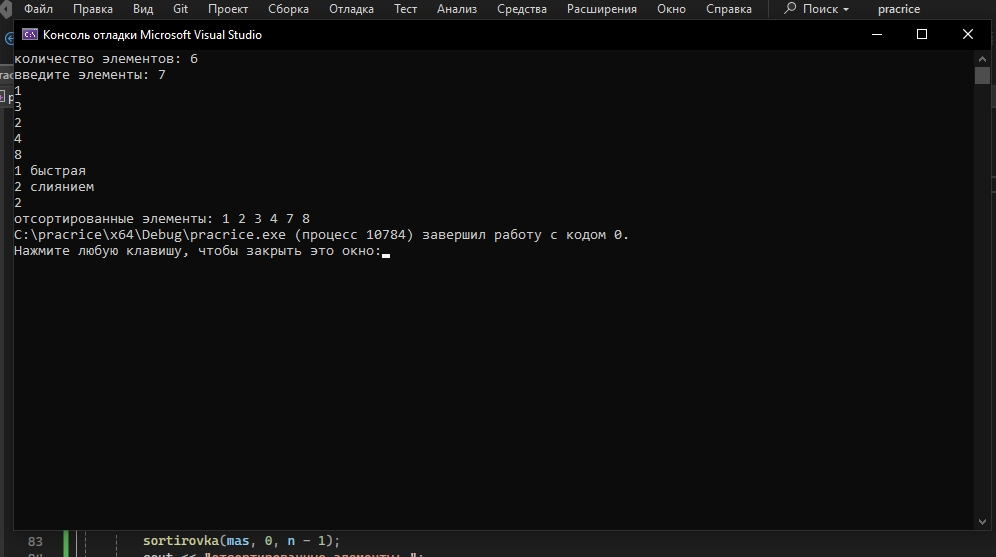
\includegraphics[width=1\textwidth]{skrin sli.jpg}
	\caption{Cортировка слиянием}\label{figure2:screen}
	\end{figure}

	\begin{thebibliography}{9}
	\bibitem{Knuth-2003}Кнут Д.Э. Всё про \TeX. \newblock --- Москва: Изд. Вильямс, 2003 г. 550~с.
	\bibitem{Lvovsky-2003}Львовский С.М. Набор и верстка в системе \LaTeX{}. \newblock --- 3-е издание, исправленное и дополненное, 2003 г.
	\bibitem{Voroncov-2005}Воронцов К.В. \LaTeX{} в примерах. 2005 г.
	\bibitem{Shildt-2013}Шилдт Г. С++ для начинающих. Шаг за шагом //ЭКОМ Паблишерз. – 2013. – №. 2. – С. 640.

	\end{thebibliography}
	
\end{document}
